(would be cool here to have just a picture you took of speckle)
\begin{figure}[ht]
\centering
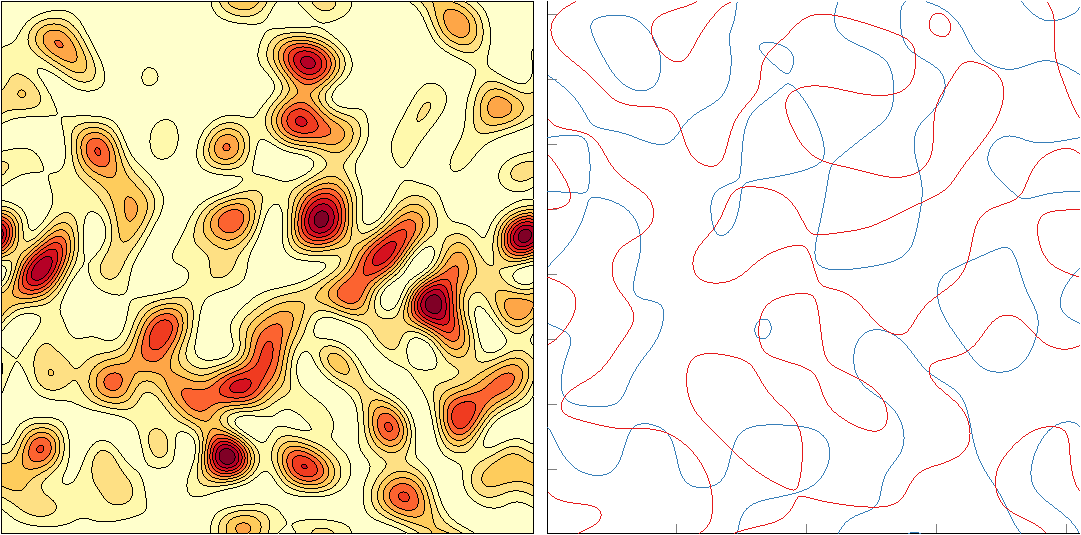
\includegraphics[keepaspectratio,width=15cm]{speckle/figures/introfig.pdf}
% ~/getvortex/specklefield.m
% make the colorbars below
\caption{Paragon speckle field, produced by the Fourier transform method.
								Right: speckle intensity.  Left: contours of the zeros of the real
								and imaginary components of the complex field, intersections of
								which are locations of optical vorticies.}
\label{fig:examplespeckle}
\end{figure}

Intro here, start in a general sense using UCF and say that optcal speckle
is just an analog of this.  \cite{lee1985universal}
In optics, the interference of coherent waves with randomly distributed
amplitudes and phases gives rise to a distincitive phenomena known as
\textit{speckle}.  An example of such is shown in
\Figure{fig:examplespeckle}.  

In this chapter we will explore the appearance of speckle in the cone, it's
properties, and how they compare with traditional speckle.
